\documentclass{article}

\usepackage{a4}
\usepackage{amsmath}
\usepackage{amsfonts}
\usepackage{amssymb}
\usepackage{float}
\usepackage[utf8]{inputenc}
\usepackage[T1]{fontenc}

\usepackage{framed}

\usepackage{graphicx}
\usepackage{caption}
\usepackage{subcaption}
\usepackage{wrapfig}

\usepackage{geometry}


\usepackage{fullpage,graphicx}
\usepackage{rotating}

\usepackage{multirow}

%\setlength{\hoffset}{-18pt}
\setlength{\oddsidemargin}{0cm}     % Marge gauche sur pages impaires
\setlength{\evensidemargin}{0cm}    % Marge gauche sur pages paires
\setlength{\marginparwidth}{54pt}   % Largeur de note dans la marge
\setlength{\textwidth}{17cm}       % Largeur de la zone de texte (17cm)
\setlength{\marginparsep}{7pt}      % Séparation de la marge
\setlength{\topmargin}{-1cm}         % Pas de marge en haut
\setlength{\headheight}{0cm}       % Haut de page
\setlength{\headsep}{10pt}          % Entre le haut de page et le texte
\setlength{\footskip}{27pt}         % Bas de page + séparation
\setlength{\textheight}{23cm}      % Hauteur de la zone de texte (25cm)

\setlength{\parskip}{1ex}
\setlength{\parindent}{1cm}

%\setlength{\topsep}{500pt}
\setlength{\abovecaptionskip}{0.1cm}
\setlength{\belowcaptionskip}{0.5cm}



\newlength{\leftbarwidth}
\setlength{\leftbarwidth}{3pt}
\newlength{\leftbarsep}
\setlength{\leftbarsep}{10pt}
\newlength{\leftbarmargin}
\setlength{\leftbarmargin}{0pt}
\newlength{\defaultparindent}
\setlength{\defaultparindent}{\parindent}


\renewenvironment{leftbar}{%
    \def\FrameCommand{\hspace{\leftbarmargin} \vrule width \leftbarwidth \relax\hspace{\leftbarsep}}%
    \MakeFramed {\advance \hsize -\width \FrameRestore }%
}{%
    \endMakeFramed
}


%\newenvironment{defx}{\noindent \\ \textbf{Definition:} \vspace{-11pt} \begin{leftbar} \vspace{4pt}}{\end{leftbar}}
%\newenvironment{propx}{\noindent \\ \textbf{Proposition:} \vspace{-11pt} \begin{framed}}{\end{framed}}

\newenvironment{defx}{
\setlength{\leftbarwidth}{3pt} 
\setlength{\leftbarmargin}{-2pt} 
\setlength{\leftbarsep}{10pt} 
\begin{leftbar}}{\end{leftbar}}
\newenvironment{propx}{\begin{framed}}{\end{framed}}

\newenvironment{demox}{\footnotesize \noindent \textit{Demo:}  \vspace{-9pt} 
\setlength{\leftbarwidth}{1pt} 
\setlength{\leftbarmargin}{5pt}
\setlength{\leftbarsep}{3pt} 
\setlength{\parindent}{7pt}

\begin{leftbar}}{\end{leftbar}
\setlength{\parindent}{\defaultparindent}
\normalsize}



\newenvironment{deft}[1]{\noindent \\ \textbf{\textsc{#1}} \vspace{-11pt} \setlength{\leftbarwidth}{3pt} 
\setlength{\leftbarmargin}{-2pt} 
\setlength{\leftbarsep}{10pt} 
\begin{leftbar} \vspace{4pt}}{\end{leftbar}}
\newenvironment{propt}[1]{\noindent \\ \textbf{\textsc{#1}} \vspace{-11pt} \begin{framed}}{ \end{framed}}


\newenvironment{algot}[1]{\noindent \\ \textbf{\textsc{#1}} \par \nobreak \vspace{1pt}\hrule\vspace{0pt} \setlength{\parindent}{0cm} \ttfamily} {\normalfont \setlength{\parindent}{\defaultparindent} \par \nobreak \vspace{4pt}\hrule\vspace{15pt}}

\newenvironment{algox}{\noindent \\  \par \nobreak \vspace{1pt}\hrule\vspace{0pt} \setlength{\parindent}{0cm} \ttfamily} {\normalfont \setlength{\parindent}{\defaultparindent} \par \nobreak \vspace{4pt}\hrule\vspace{15pt}}

%\newenvironment{algot}[1]{\noindent \\ \textbf{\textsc{#1}} \par \nobreak \vspace{1pt}\hrule\vspace{0pt} \setlength{\parindent}{0cm} \ttfamily \begin{tabbing} ~~~~\=~~~~\=~~~~\=~~~~\=~~~~\=~~~~\=~~~~} {\end{tabbing} \normalfont \setlength{\parindent}{\defaultparindent} \par \nobreak \vspace{4pt}\hrule \\}

\newcommand{\comment}[1]{\hfill// #1}

\newcommand{\bbB}{\mathbb{B}}
\newcommand{\bbN}{\mathbb{N}}
\newcommand{\bbZ}{\mathbb{Z}}
\newcommand{\bbR}{\mathbb{R}}

\newcommand{\tb}{.~~~~}

%\newcommand{\exsubpart}[1]{\subsection*{#1)}\\ }
\newcommand{\exsubpart}[1]{\subsection*{#1)} \vspace{-51pt} ~\\}

\newcommand{\info}[1]{\small{\textit{(#1)}}}




\begin{document}

\noindent {\fontsize{20}{20}\selectfont \noindent \textbf{Laboratoire d'électronique~:}}

\noindent {\fontsize{30}{30}\selectfont \noindent \textbf{Convertisseurs A/N et N/A}}

\vspace{5pt}\hrule\vspace{2pt}

\noindent {\Large \textbf{\textsc{Masur} Jonathan}\hfill \textbf{\textsc{Gosselin} Paul}}

\vspace{20pt}


On s'intéresse ici à l'étude de convertisseurs analogique/numérique (aussi appelé ``CAN'' ou ``ADC'' --- pour ``\textit{Analog-to-Digital Converter}'') et numérique/analogique (aussi appelé ``CNA'' ou ``DAC'' --- pour ``\textit{Digital-to-Analog Converter}'').

\section{Le convertisseur analogique/numérique ADC0820}
\label{sec:ADC0820}

\subsection{Prévisions théoriques}

\exsubpart{1}

Les convertisseurs analogique/numérique flash sont fréquemment utilisés, % où ?
 parce qu'ils permettent des fréquences de fonctionnement élevées. Toutefois, il se caractérisent en revanche généralement par des coûts énergétiques et spatiaux élevés.

Le principe d'un CAN flash $n$ bits est le suivant.
Supposons que les valeurs analogiques à convertir soient comprises entre deux tensions de référence $V_{min}$ et $V_{max}$, fournies au convertisseur. 
$2^n$ résistances permettent de diviser $[V_{min},V_{max}]$ en $2^n$ sous-ensembles $([V_{i-1},V_i])_{i\in[1..2^n]}$ ($V_0=V_{min}$, $V_{2^n}=V_{max}$, $\forall i\in[1..2^n], V_i> V_{i-1}$), en fournissant les $2^n-1$ tensions de transition $V_i$.
$2^n-1$ comparateurs permettent alors de situer la tension d'entrée $V_{in}$ par rapport à ces $2^n-1$ tensions de transition $V_i$.
Un encodeur $n$ bits --- entièrement numérique donc --- permet alors de convertir les sorties de ces comparateurs ($2^n-1$ bits) en l'entier $i$ correspondant sur $n$ bits~: $V_{in}\in[V_{i-1},V_i]$.

\begin{figure}[h]
  \centering
  \begin{subfigure}[b]{0.4\textwidth}
    \centering
    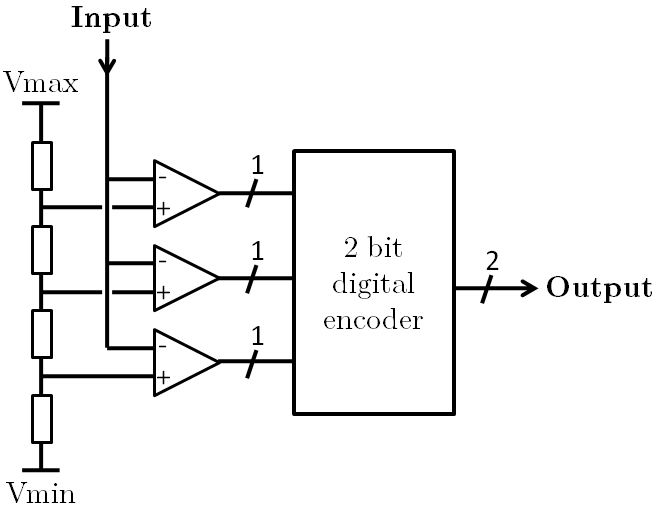
\includegraphics[width=\textwidth]{2bitFlash}
    \caption{CAN flash 2 bits}
    \label{fig:flash}
  \end{subfigure}
  ~~~~~~~~
  \begin{subfigure}[b]{0.4\textwidth}
    \centering
    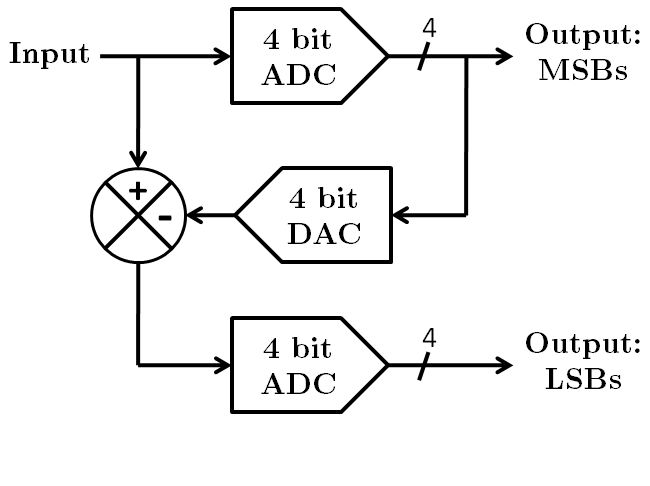
\includegraphics[width=\textwidth]{8bitSemiFlash}
    \caption{CAN semi-flash 8 bits}
    \label{fig:semiflash}
  \end{subfigure}
  \caption{Principes de base des CAN flash et semi-flash}
\end{figure}

Le principal inconvénient d'une telle structure réside dans le nombre élevé de composants utilisés. 

Pour limiter le nombre de comparateurs les convertisseurs semi-flash utilisent plusieurs convertisseurs flash. Typiquement, un convertisseur semi-flash 8 bits utilisera tout d'abord un convertisseur flash 4 bits afin d'encoder les 4 bits de poids fort (ou ``MSBs''~: ``\textit{Most Significant Bits}''). La tension $V_{MSB}$ correspondante au résultat fourni par ce convertisseur est alors soustraite à la tension d'entrée $V_{in}$, puis $V_{in}-V_{MSB}$ est traitée par un second convertisseur flash 4 bits afin d'obtenir les 4 bits de poids faible (ou ``LSBs''~: ``\textit{Less Significant Bits}'').

La réactivité du convertisseur est ainsi diminuée par rapport à un convertisseur flash d'un facteur légèrement supérieur à 2, mais le nombre de composants nécessaire passe de $O(2^n)$ à $O(2^{n/2})$.

Le convertisseur analogique/numérique utilisé dans ce travail est un CAN semi-flash 8 bits~: l'ADC0820.


\exsubpart{2}

Idéalement, l'intervalle $[V_{min},V_{max}]$ est subdivisé en intervalles identiques. Les tensions de transitions d'une valeur à l'autre en sortie du CAN sont donc données par la formule~:
\begin{equation*}
\forall i\in[1..2^n-1], V_i = V_{min}+i\cdot\frac{V_{max}-V_{min}}{2^n}
\end{equation*}
(On rappelle que $V_i$ est la tension de transition des entiers $i-1$ à $i$ en sortie du CAN.)

Dans le cadre de notre expérience~: $V_{min}=0$ et $V_{max}=V_{ref}=\mathrm{5 V}$. Ainsi~:
\begin{equation*}
\forall i\in[1..2^8-1], V_i = i\cdot\frac{V_{ref}}{2^8} = i\cdot \mathrm{19,531 mV}
\end{equation*}

Les valeurs de $V_i$ correspondantes ont été rajoutées au tableau~\ref{tab:ADC0820} des résultats expérimentaux.


\subsection{Mesures}

\exsubpart{1}

La tension d'alimentation utilisée pour le convertisseur, servant aussi de tension de référence $V_{ref}$, est fournie par une alimentation stabilisée. Elle est précisément de~: ${V_{ref}=\mathrm{4.997 V}}$.


\exsubpart{2,3}

À l'aide d'un potentiomètre 10 tours, on fait varier la tension d'entrée $V_{in}$ du CAN étudié afin de mesurer les tensions de transition $V_i$, pour lesquelles le nombre en sortie du convertisseur --- représenté en binaire par des LEDs --- passe de $i-1$ à $i$. % Plutôt de i à i+1 ?!? %

\begin{table}[h]
\caption{Résultats obtenus lors de l'étude du convertisseur ADC0820}
\label{tab:ADC0820}
\centering
\begin{tabular}{|c|c|c|c|c|c|c|c|}
\hline
$i$             & 0 & 1 & 2 & 3 & 4 & 5 & 6\\
\hline
$V_i$ théorique (V) & 0,02 & 0,039 & 0,059 & 0,078 & 0,098 & 0,117 & 0,137 \\
\hline
$V_i$ mesuré (V)    & 0,012 & 0,033 & 0,05 & 0,073 & 0,089 & 0,111 & 0.128 \\
\hline
$(V_i-V_{i-1})$ mesuré (V) & --- & 0,021 & 0,017 & 0,023 & 0,016 & 0,022 & 0,017\\
\hline
\end{tabular}

\vspace{10pt}

\begin{tabular}{|c|c|c|c|c|c|c|c|}
\hline
$i$             & 121 & 122 & 123 & 124 & 125 & 126 & 127 \\
\hline
$V_i$ théorique (V) & 2,381 & 2,401 & 2,42 & 2,44 & 2,459 & 2,479 & 2,499 \\
\hline
$V_i$ mesuré (V)    & 2,371 & 2,386 & 2,411 & 2,427 & 2,449 & 2,466 & 2,486 \\
\hline
$(V_i-V_{i-1})$ mesuré (V) & --- & 0,015 & 0,025 & 0,016 & 0,022 & 0,017 & 0,02 \\
\hline
\end{tabular}

\begin{tabular}{|c|c|c|c|c|c|c|c|}
\hline
$i$             & 128 & 129 & 130 & 131 & 132 & 133 & 134 \\
\hline
$V_i$ théorique (V) & 2,518 & 2,538 & 2,557 & 2,577 & 2,596 & 2,616 & 2,635 \\
\hline
$V_i$ mesuré (V)    & 2,507 & 2,529 & 2,544 & 2,567 & 2,583 & 2,606 & 2,622 \\
\hline
$(V_i-V_{i-1})$ mesuré (V) & 0,021 & 0,022 & 0,015 & 0,023 & 0,016 & 0,023 & 0,016 \\
\hline
\end{tabular}

\vspace{10pt}

\begin{tabular}{|c|c|c|c|c|c|}
\hline
$i$             & 250 & 251 & 252 & 253 & 254 \\
\hline
$V_i$ théorique (V) & 4,899 & 4,919 & 4,938 & 4,958 & 4,977 \\
\hline
$V_i$ mesuré (V)    & 4,883 & 4,907 & 4,922 & 4,944 & 4,961 \\
\hline
$(V_i-V_{i-1})$ mesuré (V) & --- & 0,024 & 0,015 & 0,022 & 0,017 \\
\hline
\end{tabular}
\end{table}

Ces résultats, comparés aux résultats théoriques donnés par ${V_i = i\cdot\frac{V_{ref}}{2^8}}$ et ${V_{ref}=4,997\mathrm{V}}$ sont représentés Fig.~\ref{fig:ADCres1}.

\begin{figure}
  \centering
  \begin{subfigure}[b]{\textwidth}
    \centering
    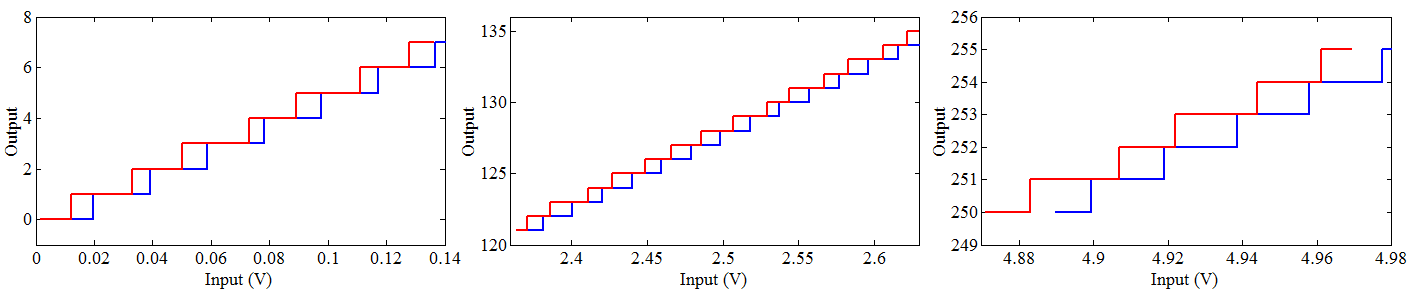
\includegraphics[width=\textwidth]{ADCresults}
    \caption{Résultats obtenus (en rouge), comparés à ${V_i = i\cdot\frac{V_{ref}}{2^8}}$ (en bleu) (${V_{ref}=4,997\mathrm{V}}$)}
    \label{fig:ADCres1}
  \end{subfigure}
  \\
  \begin{subfigure}[b]{\textwidth}
    \centering
    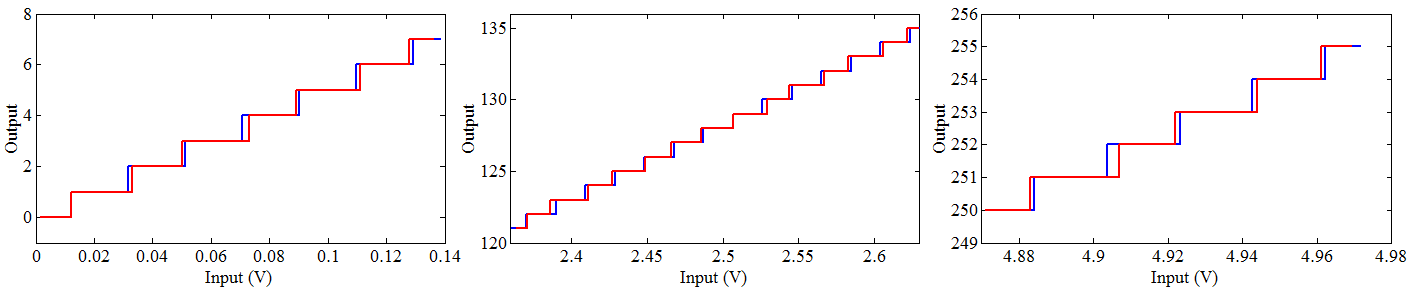
\includegraphics[width=\textwidth]{ADCresults_lincorr}
    \caption{Résultats obtenus (en rouge), comparés à ${V_i = V_{min}+i\cdot\frac{V_{max}-V_{min}}{2^n}}$ (en bleu) (${V_{min}=-0,0073\mathrm{V}}$, ${V_{max}=4,9816\mathrm{V}}$)}
    \label{fig:ADCres2}
  \end{subfigure}
  \\
  \begin{subfigure}[b]{\textwidth}
    \centering
    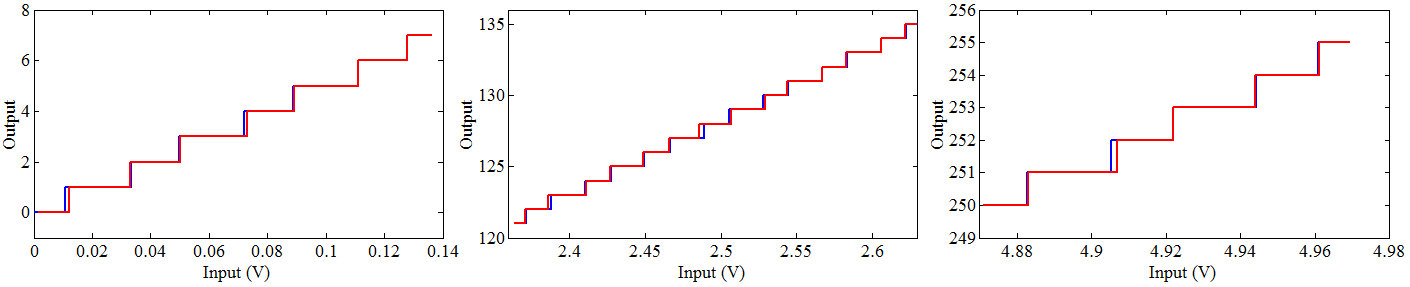
\includegraphics[width=\textwidth]{ADCresults_corr}
    \caption{Résultats obtenus (en rouge), comparés à ${V_i = V_{min}+i\cdot\frac{V_{max}-V_{min}}{2^n}}+p_i\delta V$ (en bleu) \\(${V_{min}=-0,0072\mathrm{V}}$, ${V_{max}=4,9817\mathrm{V}}$, ${\delta V=0,0015\mathrm{V}}$)}
    \label{fig:ADCres3}
  \end{subfigure}
  \caption{Résultat obtenu avec le convertisseur analogique/numérique ADC0820}
  \label{fig:ADCres}
\end{figure}

% % Clarifier un peu STP

La première chose que l'on observe est un décalage permanent entre les valeurs de $V_i$ mesurées (que l'on notera $V_i^{mes}$) et les valeurs de $V_i$ théorique (que l'on notera $V_i^{th}$). On constate en effet un $offset$ moyen de $-0,0111$. On remarque toutefois que $V_i^{mes}-V_i^{th}$ augmente avec $i$ (${\langle V_i^{mes}-V_i^{th}\rangle_{i\in[1..7]}=-0,0072}$, ${\langle V_i^{mes}-V_i^{th}\rangle_{i\in[122..135]}=-0,0115}$, ${\langle V_i^{mes}-V_i^{th}\rangle_{i\in[251..255]}=-0,0150}$). 

Afin d'obtenir une meilleure approximation des résultats pratiques, on peut réutiliser la formule~:
\begin{equation*}
V_i^{th} = V_{min}+i\cdot\frac{V_{max}-V_{min}}{2^n}
\end{equation*}

On a calculé via Matlab les valeurs optimales pour $V_{min}$ et $V_{max}$ \footnote{Valeurs minimisant $\sum (V_i^{mes}-V_i^{th})^2$}, et obtenu~: ${V_{min}=-0,0073\mathrm{V}}$, ${V_{min}=4,9816\mathrm{V}}$. Les résultats correspondants sont présentés Fig.~\ref{fig:ADCres2}.

On remarque par ailleurs que pour $i$ pair $(V_i^{mes}-V_{i-1}^{mes})$ est généralement de l'ordre de $0,016\mathrm{V}$, tandis que cette valeur est généralement de l'ordre de $0,022\mathrm{V}$ pour $i$ impair. Pour représenter cette effet de la parité de $i$ sur $V_i$, on pourra utiliser la modélisation~: 
\begin{equation*}
V_i^{th} = V_{min}+i\cdot\frac{V_{max}-V_{min}}{2^n}+p_i\delta V \mathrm{~~~~avec~:~~}p_i = \begin{cases} +1 &\mathrm{si~} i\in 2\bbN \\ -1 & \mbox{sinon}\end{cases}
\end{equation*}

Là encore, on obtient avec Matlab les coefficients optimum~: ${V_{min}=-0,0072\mathrm{V}}$, ${V_{max}=4,9817\mathrm{V}}$, \\${\delta V=0,0015\mathrm{V}}$. Les résultats correspondants sont présentés Fig.~\ref{fig:ADCres3}.



Nous avons tenté de comprendre l'origine de cet effet de la parité de $i$ sur la tension de transition $V_i$. Compte tenu du principe de fonctionnement du convertisseur semi-flash, cet effet ne peut être imputé au calcul du bit de poids faible. En effet, ce dernier est donné par l'encodeur numérique encodant les quatre bits de poids faible. Il ne peut pas non plus être imputé au convertisseur numérique/analogique interne du convertisseur analogie/numérique étudié~: en effet, la sortie de ce convertisseur numérique/analogique n'est modifiée que lorsqu'un des quatre bits de poids fort est modifié. 

On en déduit que le problème est lié aux quinze ($2^4-1$) comparateurs fournissant les bits en entrée de l'encodeur 4-bits des bits de poids faibles. Leurs offsets seraient quasiment identiques pour les tensions de seuil $V_i$ avec $i$ pair, ainsi que pour les tensions de seuil $V_i$ avec $i$ impair.

L'hypothèse réalisée est la suivante~: tous les comparateurs utilisés ont un offset quasiment égal à $\delta V$ --- ce qui ce justifie en pratique~: cet offset est fortement lié au substrat, dont les caractéristiques peuvent être considérées comme constantes au sein du convertisseur étudié. En revanche, un convertisseur sur deux serait placé ``à l'envers''~: on code ${V < V_i}$ pour $i$ pair, et ${V > V_i}$ pour $i$ impair (ou l'inverse). Cela se justifie par une éventuelle simplification de l'encodeur 4-bits obtenue en codant un bit sur deux en entrée avec une logique négative.


\section{Le convertisseur numérique/analogique AD7524}
\label{sec:AD7524}

\subsection{Prévisions théoriques}

\exsubpart{1}

Le convertisseur numérique/analogique étudié est un CNA 8 bits à réseau R/2R : l'AD7524.

Le principe de base de la plupart des CNA à réseau R/2R repose sur l'équivalence représentée Fig.~\ref{fig:R2Rbase1}, où $V_{min}$ et $V_{max}$ sont des tensions fixées. De cette équivalence découle l'équivalence représentée Fig.~\ref{fig:R2Rbase2}, où $V_{ref}$ est une tension fixée, $B_0$, $B_1$, \dots, $B_{n-1}$ sont les bits en entrée du CNA, et~:
\begin{equation*}
V_{eq} = \left(\sum_{i=0}^{n-1}\frac{1}{2^{n-i}}B_i\right)V_{ref}
\end{equation*}

\begin{figure}[h]
  \centering
  \begin{subfigure}[b]{0.43\textwidth}
    \centering
    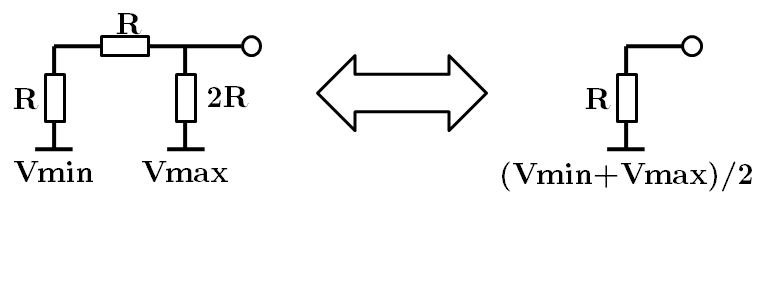
\includegraphics[width=\textwidth]{R2Rbasics}
    \caption{Équivalence de base}
    \label{fig:R2Rbase1}
  \end{subfigure}
  ~~~~
  \begin{subfigure}[b]{0.53\textwidth}
    \centering
    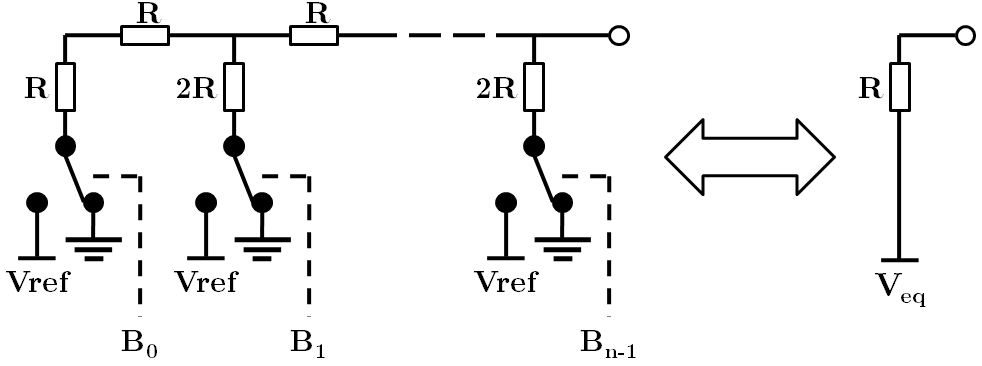
\includegraphics[width=\textwidth]{R2Rexpended}
    \caption{Équivalence en résultant}
    \label{fig:R2Rbase2}
  \end{subfigure}
  \caption{Principe de base des CNA à réseau R/2R}
\end{figure}

On utilise alors généralement un amplificateur opérationnel branché en suiveur ou en amplificateur de gain $-1$, afin d'obtenir en sortie la tension $V_{eq}$ indépendamment du reste du circuit.


Le fonctionnement de l'AD7524 est légèrement différent. Le circuit correspondant, tel qu'il est branché (avec notamment la sortie OUT2 branchée à la masse et l'utilisation d'un amplificateur opérationnel), est représenté Fig.~\ref{fig:AD7524} \footnote{Un condensateur, liant $V_{out1}$ et $V_{out}$, a été omis~: proposé par les datasheets, son but est d'empêcher des oscillations en sortie de l'amplificateur opérationnel. Nous nous plaçons dans le cadre d'un état déjà stabilisé, où le condensateur agit comme un interrupteur ouvert.}
% Je ne comprends pas cette note - les condensateurs sont présent dans le shéma compelet}.

\begin{figure}[h]
  \centering
  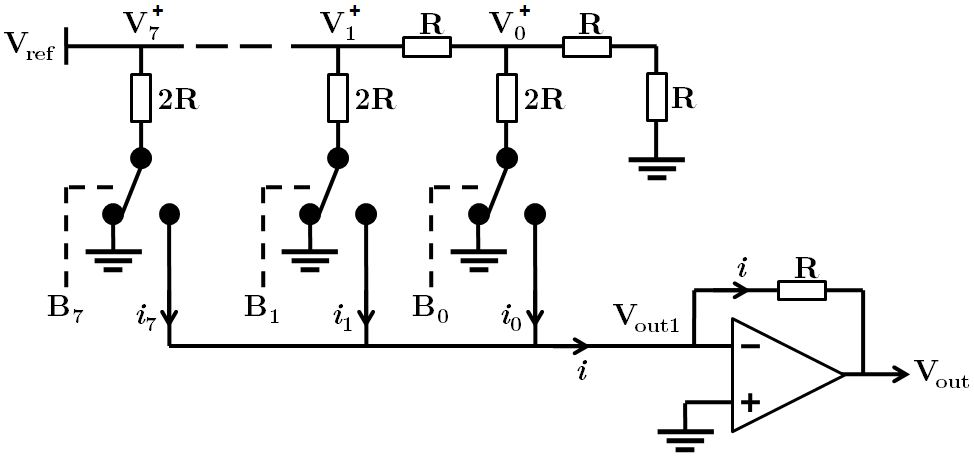
\includegraphics[width=.6\textwidth]{AD7524}
  \caption{Le convertisseur AD7524 en situation}
  \label{fig:AD7524}
\end{figure}

\begin{wrapfigure}{r}{0.3\textwidth}
  \begin{center}
    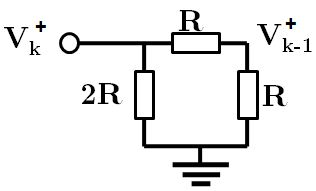
\includegraphics[width=0.2\textwidth]{AD7524eq}
  \end{center}
  \caption{Calcul des $V_k^+$}
  \label{fig:AD7524eq}
\end{wrapfigure}

L'amplificateur opérationnel fixe $V_{out1}=0$. L'équivalence présentée Fig.~\ref{fig:R2Rbase1} permet alors de calculer par récurrence les tenions $V_k^+$ (cf Fig.~\ref{fig:AD7524eq})~: $V_7^+ = V_{ref}$ et $V_{k-1}^+=\frac{V_k^+}{2}$~; d'où~: ${V_k^+=\frac{V_{ref}}{2^{7-k}}}$.

On obtient alors~:
\begin{equation*}
i = \sum_{k=0}^7 i_k = \sum_{k=0}^7 B_k \frac{V_k^+}{2R} = \frac{V_{ref}}{R} \sum_{k=0}^7 \frac{1}{2^{8-k}} B_k
\end{equation*}


Puisque $V_{out} = -R~i$, dans notre cas, on obtient ainsi pour l'ensemble des bits d'entrée $(B_0,\dots,B_7)$ un tension de sortie donnée par la formule~:
\begin{equation}
V_{out}(B_0\dots B_7) = -\left(\sum_{k=0}^{7}\frac{1}{2^{n-k}}B_k\right)V_{ref}
\label{eq:CNAeq}
\end{equation}

\exsubpart{2}

Selon la formule~\ref{eq:CNAeq}, la contribution du bit $i$ à la tension de sortie $V_{out}$ est donnée par la formule~:
\begin{equation*}
V_i^{out} = -\frac{1}{2^{8-i}}V_{ref}
\end{equation*}

Les valeurs correspondantes ont été rajoutées au tableau~\ref{tab:AD7524} des résultats théoriques.

\exsubpart{3}

Toujours selon la formule~\ref{eq:CNAeq}, on a théoriquement~:
\begin{equation*}
V_{out}(\mathtt{00000000_b}) = 0
\end{equation*}
et~:
\begin{eqnarray*}
V_{out}(\mathtt{11111111_b}) &=& -\left(\sum_{i=0}^{7}\frac{1}{2^{8-i}}B_i\right)V_{ref} = -(1-\frac{1}{2^8})V_{ref}\\
V_{out}(\mathtt{11111111_b}) &=& -4,9775\mathrm{V}
\end{eqnarray*}


\subsection{Mesures}

\exsubpart{1}

Cette fois encore, la tension d'alimentation utilisée pour le convertisseur, servant aussi de tension de référence $V_{ref}$, est fournie par une alimentation stabilisée~; et est précisément de~: ${V_{ref}=\mathrm{4.997 V}}$.


\exsubpart{2,3}

Expérimentalement, on mesure la contribution $V_i^{out}$ de chaque bit $i$ en mettant en entrée du CNA tous les bits à zéro, excepté le bit $i$. Ainsi, on considère~:
\begin{equation*}
V_i^{out} = V_{out}(\delta_{0,i}\delta_{1,i}\delta_{2,i}\delta_{3,i}\delta_{4,i}\delta_{5,i}\delta_{6,i}\delta_{7,i}) \mathrm{~~~~avec~:~~}\delta_{j,i} = \begin{cases} \mathtt{1} &\mathrm{si~} i=j \\ \mathtt{0} & \mbox{sinon}\end{cases}
\end{equation*}

Les résultats obtenus sont présentés dans le tableau~\ref{tab:AD7524}. $V_i^{out,th}$ désigne la valeur théorique de la contribution du bit $i$ à la tension de sortie $V_{out}$, tandis que $V_i^{out,mes}$ en désigne la valeur mesurée expérimentalement.



\begin{table}[h]
\caption{Résultats obtenus lors de l'étude du convertisseur AD7524}
\label{tab:AD7524}
\centering
% Ce tableau n'est pas clair - a quoi correspond chaque ligne ??

\begin{tabular}{|c|c|c|c|c|c|c|c|c|}
\hline
$i$ & 0 & 1 & 2 & 3 & 4 & 5 & 6 & 7 \\
\hline
$V_i^{out,th}$ (V) & -0,0195 & -0,039 & -0,0781 & -0,1562 & -0,3123 & -0,6246 & -1,2493 & -2,4985 \\
\hline
$V_i^{out,mes}$ (V) & -0,019 & -0,039 & -0,078 & -0,157 & -0,314 & -0,628 & -1,258 & -2,518 \\
\hline
$\sum_{j\leq i}V_j^{out,mes}$ (V) & -0,019 & -0,058 & -0,136 & -0,293 & -0,607 & -1,235 & -2,493 & -5,011 \\
\hline
\end{tabular}

%\vspace{10pt}

\subsubsection{Tension de sortie pour les codes d'entrée minimum et maxium}


\begin{tabular}{|c|c|c|}
\hline
Entrée & \texttt{$00000000_b$} & \texttt{$11111111_b$} \\
\hline
$V_{out}$ théorique (V) & 0 & -4,9775 \\
\hline
$V_{out}$ mesurée (V) & 0,001 & -5,04 \\
\hline
\end{tabular}
\end{table}

On remarque que l'on a notamment~: $\forall i\in [1..7], \sum_{j<i}V_j^{out,mes} < V_i^{out,mes}$.

Ainsi, le convertisseur numérique/analogique étudié est monotone. En effet, cela montre que si ${\forall j>i, B'_j=B_j}$, $B_i=0$, $B'_i=1$, ${\forall j<i, B_j=1}$ et ${\forall j<i, B'_j=0}$, alors~: \begin{equation*}V_i^{out,mes}(B_7B_6B_5B_4B_3B_2B_1B_0) < V_i^{out,mes}(B'_7B'_6B'_5B'_4B'_3B'_2B'_1B'_0)\end{equation*} \\(Par exemple~: $V_i^{out,mes}(B_7B_6B_5B_4\mathtt{0111}) < V_i^{out,mes}(B'_7B'_6B'_5B'_4\mathtt{1000})$.)

Les écarts entre les valeurs théoriques et mesurées pour $V_{out}(\mathtt{00000000})$ et $V_{out}(\mathtt{11111111})$ s'explique notamment par une légère différence entre les résistances liant les sorties OUT1 et R\_FDBK au sein du convertisseur AD7524, ainsi que par les imperfections de l'amplificateur opérationnel (offset et gain fini). De ces imperfections, il résulte un offset en sortie de l'ensemble du convertisseur, amplificateur opérationnel inclus, ainsi qu'une erreur sur le gain.

L'offset est donné par~: 
\begin{equation*}
V_{offset}=V_{out}^{mes}(\mathtt{00000000})-V_{out}^{th}(\mathtt{00000000})=0,001\mathrm{V}
\end{equation*}
et l'erreur sur le gain est donnée par~:
\begin{equation*}
\delta_G=\frac{(V_{out}^{mes}(\mathtt{11111111})-V_{out}^{mes}(\mathtt{00000000}))-(V_{out}^{th}(\mathtt{11111111})-V_{out}^{th}(\mathtt{00000000}))}{V_{out}^{th}(\mathtt{11111111})-V_{out}^{th}(\mathtt{00000000})}=1,25\mathrm{\%}
\end{equation*}

On peut alors préciser la formule fournissant $V_{out}$, en prenant~:
\begin{equation*}
V_{out}^{th}(B_0\dots B_7) = V_{offset}-(1+\delta_G)\left(\sum_{k=0}^{7}\frac{1}{2^{n-k}}B_k\right)V_{ref} = V_{offset}-\left(\sum_{k=0}^{7}\frac{1}{2^{n-k}}B_k\right)\widetilde{V_{ref}}
\end{equation*}
avec~: $\widetilde{V_{ref}} = (1+\delta_G)V_{ref} = -\frac{V_{out}^{mes}(\mathtt{11111111})-V_{out}^{mes}(\mathtt{00000000})}{1-\frac{1}{2^8}} = 5,061\mathrm{V}$



\section{Chaine de conversion A/N - N/A}


\subsection{Montage étudié}

On connecte maintenant les 8 bits de sortie du convertisseur analogique/numérique ADC0820 étudié section~\ref{sec:ADC0820} aux 8 bits d'entrée du convertisseur numérique/analogique AD7524 étudié section~\ref{sec:AD7524}.

On notera $V_{in}$ la tension imposée en entrée du montage (tension d'entrée du convertisseur analogique/numérique), et $V_{out}$ la tension obtenue en sortie (tension de sortie du convertisseur numérique/analogique). 

Dans le cadre de convertisseurs parfaits, d'une fréquence d'échantillonnage infinie et d'un nombre de bits infini, on aurait donc : $V_{out}=-V_{in}$. Dans notre cas, on obtient évidemment une approximation~; et les différences entre $V_{out}$ et $-V_{in}$ seront discutées plus bas.

Pour cela, un amplificateur sommateur permet d'obtenir en plus de la sortie du montage la tension~: ${V_{err}=-(V_{out}+V_{in})}$.

\subsection{Mesures}

\exsubpart{1}

Afin d'observer les effets de la chaîne AN-NA sur le signal (échantillonnage, quantification\dots), on applique en entrée un signal $V_{in}$ triangulaire d'amplitude $4\mathrm{V}$ et de moyenne $2,5\mathrm{V}$. On en fera varier la fréquence $f_{in}$.

\noindent \textbf{\underline{Quantification}}.

Afin d'observer l'effet de la quantification, sans être perturbé par l'échantillonnage, on utilise en entrée un signal lent~: $f_{in}\ll f_{ech}$ (où $f_{ech}$ désigne la fréquence d'échantillonnage des convertisseurs, qui est de l'ordre de $20\mathrm{kHz}$). Typiquement, on utilisera ici $f_{in} = \mathrm{0,5 Hz}$.

Les résultats expérimentaux obtenus sont fournis Fig.~\ref{fig:slowT}.


Le phénomène de quantification s'observe bien lorsque l'on trace $V_{out}=f(V_{in})$ (cf. Fig.~\ref{fig:slowXY}). On y observe des ``marches'' de hauteurs et largeurs régulières, de l'ordre de $\frac{V_{ref}}{2^8}\approx\mathrm{19,5 mV}$. Ces marches sont continues sur le plan horizontal, mais pas sur le plan vertical~: à chaque valeur de $V_{out}$ correspondent plusieurs valeurs de $V_{in}$. Plus simplement, sans prendre en compte d'éventuels offsets ou erreurs de gain, lors de la conversion $V_{in}\rightarrow V_{out}$, $-V_{in}$ est ``rabattu'' sur la valeur la plus proche possible de $V_{out}$.

On introduit ainsi un erreur de quantification comprise entre $-\epsilon_q$ et $+\epsilon_q$, avec ${\epsilon_q = \frac{1}{2}\frac{V_{ref}}{2^8}}$.



\noindent \textbf{\underline{Échantillonnage}}.

%\begin{figure}[h!]
%  \centering
%  \hfill
%  \begin{subfigure}[b]{0.3\textwidth}
%    \centering
%    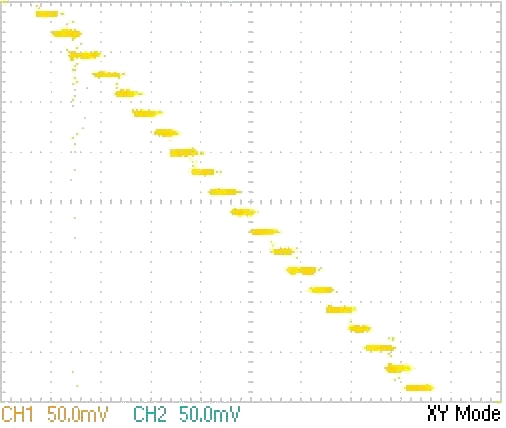
\includegraphics[width=\textwidth]{data/TEK0017_}
%    \caption{$f_{in}=$0,5 Hz)}
%    \label{fig:slowXY_}
%  \end{subfigure}
%  \hfill
%  \begin{subfigure}[b]{0.3\textwidth}
%    \centering
%    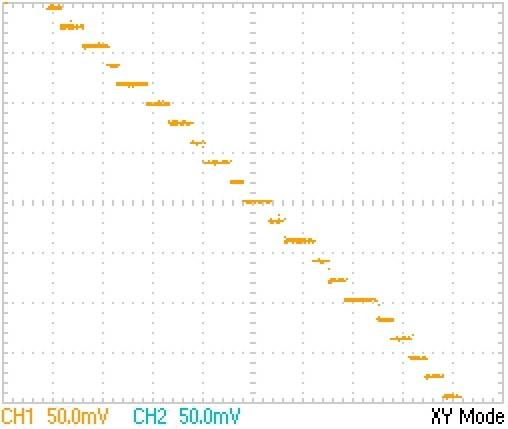
\includegraphics[width=\textwidth]{data/TEK0000_}
%    \caption{$f_{in}=$50 Hz)}
%    \label{fig:midXY}
%  \end{subfigure}
%  \hfill
%  \begin{subfigure}[b]{0.3\textwidth}
%    \centering
%    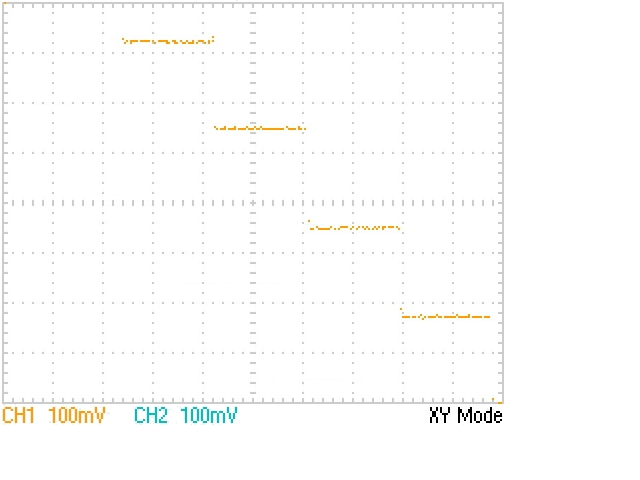
\includegraphics[width=\textwidth]{data/TEK0020_}
%    \caption{$f_{in}=$0,5 Hz)}
%    \label{fig:fastXY}
%  \end{subfigure}
%  \hfill  \caption{$V_{out}=f(V_{in})$ pour différentes fréquences d'entrées}
%  \label{fig:slow}
%\end{figure}
%
%\begin{sidewaysfigure}
%  \centering
%  \begin{subfigure}{0.28\textwidth}
%          \centering
%          \includegraphics[width=\textwidth]{pb31}
%          \caption{Basic data-flow graph}
%          \label{fig:pb31}
%  \end{subfigure}
%  ~~~
%  \begin{subfigure}{0.65\textwidth}
%    \centering
%    \begin{subfigure}{\textwidth}
%            \centering
%            \includegraphics[width=\textwidth]{pb32}
%            \caption{Reduced data-flow graph, using tree height reduction}
%            \label{fig:pb32}
%    \end{subfigure}
%    \\
%    \begin{subfigure}{0.9\textwidth}
%            \centering
%            \includegraphics[width=\textwidth]{pb33}
%            \caption{Reduced data-flow graph, using constant propagation and operator strength reduction}
%            \label{fig:pb33}
%    \end{subfigure}
%  \end{subfigure}
%  \caption{Data-flow graphs for Problem III}
%\end{sidewaysfigure}

\begin{sidewaysfigure}
	\centering
	\begin{subfigure}[b]{0.3\textwidth}
		\begin{subfigure}[b]{\textwidth}
			\centering
			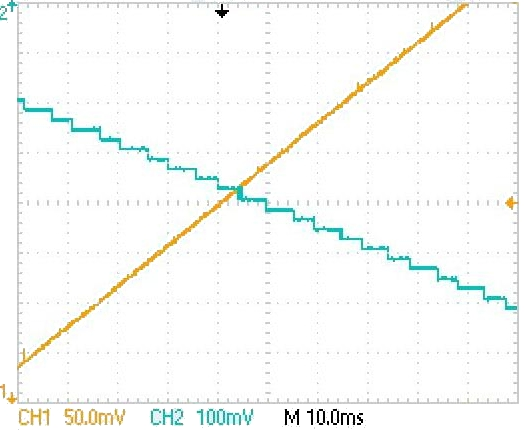
\includegraphics[width=\textwidth]{data/TEK0018_}
			\caption{\centering $f_{in}=\mathrm{0,5 Hz}$\\$V_{out}=f(t)$ (CH1), $V_{out}=f(t)$ (CH2)}
			\label{fig:slowT}
		\end{subfigure}
		\\
		\begin{subfigure}[b]{\textwidth}
			\centering
			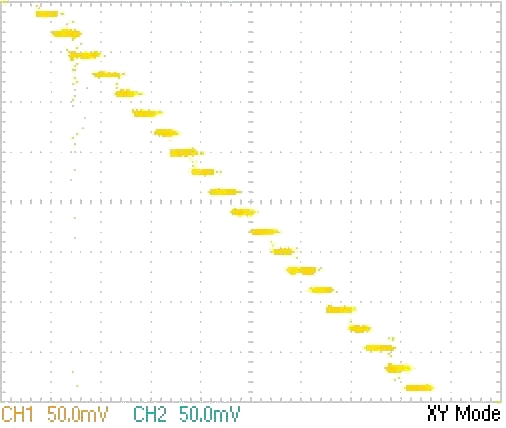
\includegraphics[width=\textwidth]{data/TEK0017_}
			\caption{\centering $f_{in}=\mathrm{0,5 Hz}$\\$V_{out}=f(V_{in})$}
			\label{fig:slowXY}
		\end{subfigure}
	\end{subfigure}
	\hfill
	\begin{subfigure}[b]{0.3\textwidth}
		\begin{subfigure}[b]{\textwidth}
			\centering
			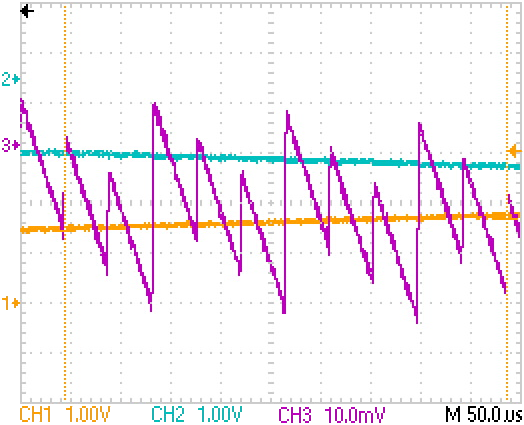
\includegraphics[width=\textwidth]{data/TEK0008_}
			\caption{\centering $f_{in}=\mathrm{60 Hz}$, $V_{out}=f(t)$ (CH1),\\ $V_{out}=f(t)$ (CH2), $V_{err}=f(t)$ (CH3)}
			\label{fig:ech1}
		\end{subfigure}
		\\
		\begin{subfigure}[b]{\textwidth}
			\centering
			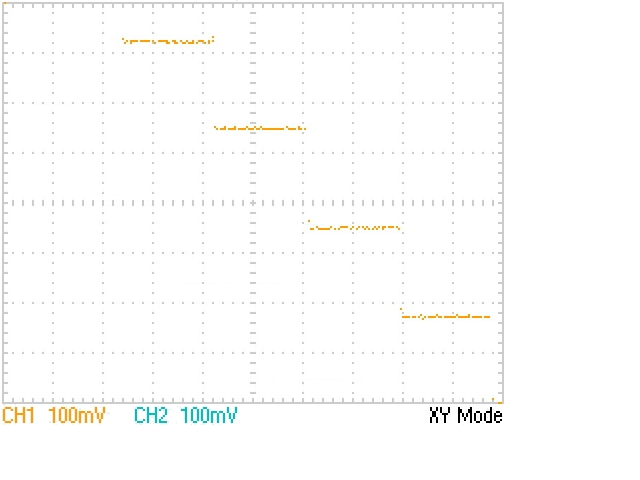
\includegraphics[width=\textwidth]{data/TEK0020_}
			\caption{\centering $f_{in}=\mathrm{500 Hz}$\\$V_{out}=f(V_{in})$}
			\label{fig:ech2}
		\end{subfigure}
	\end{subfigure}
	\hfill
	\begin{subfigure}[b]{0.3\textwidth}
		\begin{subfigure}[b]{\textwidth}
			\centering
			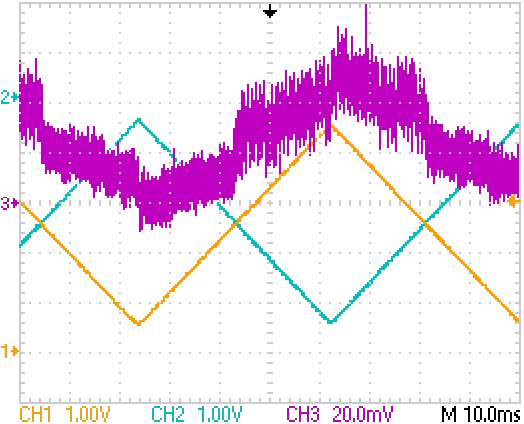
\includegraphics[width=\textwidth]{data/TEK0005_}
			\caption{\centering $f_{in}=\mathrm{13 Hz}$, $V_{out}=f(t)$ (CH1),\\ $V_{out}=f(t)$ (CH2), $V_{err}=f(t)$ (CH3)}
			\label{fig:gain}
		\end{subfigure}
		\\
		\begin{subfigure}[b]{\textwidth}
			\centering
			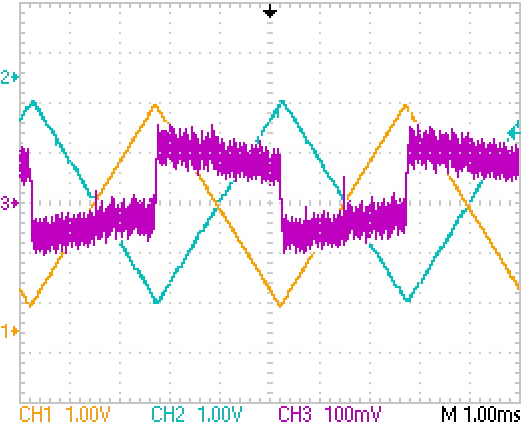
\includegraphics[width=\textwidth]{data/TEK0010_}
			\caption{\centering $f_{in}=\mathrm{200 Hz}$, $V_{out}=f(t)$ (CH1),\\ $V_{out}=f(t)$ (CH2), $V_{err}=f(t)$ (CH3)}
			\label{fig:retard}
		\end{subfigure}
	\end{subfigure}	
	\caption{Data-flow graphs for Problem III}
\end{sidewaysfigure}

Afin de pouvoir être utilisé par un système synchrone, le CAN étudié bénéficie d'un ``\textit{sample-and-hold}''~: tous les $T_{ech}$, l'entrée $V_{in}$ est mémorisée, et c'est la conversion en bits de cette valeur mémorisée qui est fournie en sortie. Ainsi, cette sortie est mise à jour avec une fréquence dite d'échantillonnage $f_{ech} = T_{ech}^{-1}$. Cette mise-à-jour périodique est observable  Fig.~\ref{fig:ech1}~: elle est à l'origine des irrégularités observées pour $V_{err}$\footnote{Lorsque la fréquence d'échantillonnage du CAN n'intervient pas (ie pour un signal d'entrée suffisamment lent), $V_{err}$ présente des dans de scies identiques (même taille, mêmes extrema).}.On peut par ailleurs mesurer sur cette figure~: ${f_{ech} = 22,5\mathrm{kHz}}$.

Pour un signal d'entrée variant à une vitesse $\frac{dV_{in}}{dt}$ constante, le retard sur l'information engendré ajoute à l'erreur de quantification une erreur pouvant atteindre ${\epsilon_{ech} = T_{ech}\frac{dV_{in}}{dt}}$. Dans le cas présenté Fig.~\ref{fig:ech1}, où ${f_{in}=60\mathrm{Hz}}$, on obtient ${\epsilon_{ech} = 22\mathrm{mV}}$ --- ce qui s'accorde avec les résultats expérimentaux, donnant~: \\${\epsilon_q+\epsilon_{ech}\approx 42\mathrm{mV}}$.

Lorsque $\epsilon_{ech}$ dépasse $\frac{V_{ref}}{2^n}$, certaines valeurs possibles pour $V_{out}$ n'ont même pas le temps d'être ``vues''. Cette situation extrêmes est représentée Fig.~\ref{fig:ech2}.


\noindent \textbf{\underline{Gain et offset}}.

Le CAN et le CNA présentant tous deux une erreur sur le gain ainsi qu'un certain offset, cela se répercute sur la chaîne étudiée --- les deux gains étant multipliés et les offset sommés. Cet effet s'observe bien à $13Hz$ (cf. Fig.~\ref{fig:gain})~: le signal $V_{err}$ obtenu est constitué d'oscillations en dans de scies (liées aux effets précédemment décrits) autours d'un signal triangulaire traduisant cette erreur de gain. Son amplitude est d'approximativement $50\mathrm{mV}$ (pour une amplitude d'entrée de $4\mathrm{V}$), ce qui traduit une erreur de gain de $1,25\%$.


\noindent \textbf{\underline{Retard}}.

Indépendamment des erreurs liées à la fréquence d'échantillonnage, la succession du CAN et du CNA engendrent irrémédiablement un retard $\delta t$ entre la sortie et l'entrée. Lorsque l'on augmente la fréquence du signal traité, la soustraction $V_{err}$ des signaux triangulaires décalés $V_{out}$ et $-V_{in}$ aboutie en un signal carré d'amplitude proportionnelle au retard, auquel s'ajoute les perturbations précédemment décrites. Cet effet est observable Fig.~\ref{fig:retard}.

Plus précisément, l'amplitude du signal carré susmentionné est de ${2 \epsilon_{retard}}$ avec ${\epsilon_{retard} = 2 \delta t \left|\frac{dV_{in}}{dt}\right|}$. Expérimentalement, on obtient pour ${f_{in}=200\mathrm{Hz}}$ (donc ${\left|\frac{dV_{in}}{dt}\right|=1600\mathrm{ V\cdot s^{-1}}}$) ${2 \epsilon_{retard} = 144\mathrm{mV}}$. Ainsi~: ${\epsilon_{retard} = 72\mathrm{mV}}$ et  ${\delta t = 22,5\mathrm{\mu s}}$.





% Erreurs :
%  - Echantillonage
%      > Verr sur fréq rapide : largeur régulière, estimation de la fréq d'échantillonage
%      > Escalier sur fréq plus rapide : marche de longueur non régulière (dVin ou 2*dVin)
%  - Gain
%      > Verr dézoomé, fréq raisonnable
%  - Retard
%      > Verr dézoomé, fréq haute : au Verr précédemment affiché, on ajoute un signal carré




















\section{Application~: la chambre d'écho}

\subsection{Prévisions théoriques}

Le principe de la chambre d'écho est d'échantillonner un signal audio à l'aide du convertisseur AN, de stocker les échantillons dans un tampon circulaire réalisé à l'aide d'une mémoire SRAM de 8-bits, puis de restituer les données passées qui sont stockées dans la mémoire à l'aide du convertisseur NA.

\begin{figure}[h]
	\centering
	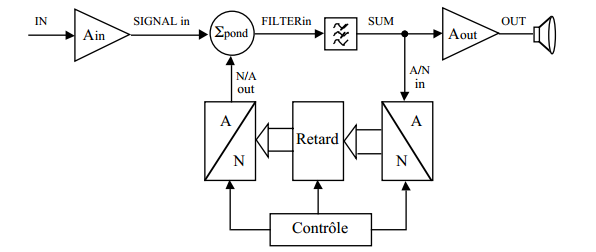
\includegraphics[width=.4\textwidth]{principe_chambre_d'echo.png}
	\caption{Schéma de principe de la chambre d'écho}
	\label{fig:chambre_echo}
\end{figure}

Il y a alors plusieurs modes de fonctionnement~:
\begin{itemize}
\item \textbf{Écho seul}~: Le signal est désactivé mais l'écho est activé. Il s'agit donc d'un simple retard.
\item \textbf{Écho simple}~: Le signal et l'écho sont activés, mais le sommateur est désactivé. Le signal est sommé avec le contenu de la mémoire, mais seul le signal est écrit dans la mémoire. Il n'y a donc qu'un seul écho.
\item \textbf{Écho infini}~: Le signal, l'écho et le sommateur sont activés. Le signal est sommé avec le contenu de la mémoire avant d'être écrit dans la mémoire. Il y a donc un feedback sur l'écho, ce qui simule mieux un écho réel.
\end{itemize}

\exsubpart{1}

Les conditions à garantir pour assurer la stabilité du système diffère du mode de fonctionnement utilisé~:

\noindent \textbf{\underline{En mode écho simple~:}}

Théoriquement, un système d'écho simple est équivalent à un filtre à réponse impulsionnelle finie (RIF), dont la réponse est~: $y[n] = x[n] + k \cdot x[n-l]$,
où $x$ désigne entrée, $y$ la sortie, $k$ le facteur d'amplification et $l$ la taille du tampon en mémoire.

Sa fonction de transfert est donc~: $H(z) = 1 + k \cdot z^l$

Il n'y a pas de pôles, le système sera toujours stable.

\noindent \textbf{\underline{En mode écho infini~:}}

Un écho infini est équivalent à un filtre à réponse impulsionnelle infinie (RII), dont la réponse est~: $y[n] = x[n] + k \cdot y[n-l]$

La fonction de transfert est donc~: $H(z) = \frac{1}{1 - k \cdot z^{-l}}$

Ce système sera stable seulement pour les $k<1$. En cas d'instabilité, la chambre d'écho ne fonctionnera pas, un régime d'oscillation apparaîtra et un sifflement fort s'entendra sur la sortie. En musique, cela correspond à ce que l'on nomme l'``effet Larsen''.
\\

À noter que la réponse en fréquence de la chambre d'écho n'est pas constante~: certaines fréquences vont être amplifiées tandis que d'autres vont être atténuées, et ce pour les deux modes écho simple et infini. Cet effet de bord est inévitable. De plus, toute modification des paramètres $k$ et $l$ va affecter la réponse en fréquence.

Cette étude de la chambre d'écho comme filtre est valable pour des retards petits devant la durée des signaux en entrées (ie $l$ petit), c'est-à-dire quand l'écho ne sera pas perçu comme tel par l'oreille humaine. Pour un retard plus grand (plus long que les notes en entrée par exemple), l'écho ne sera plus perçu comme un filtre. Toutefois, les conditions de stabilité sont inchangées~: pour un écho infini, si $k>1$, l'écho sera à chaque fois amplifié et son amplitude divergera vers $+\infty$. 

\exsubpart{2}

On désire avoir une bande passante de $15 \mathrm{kHz}$. Pour respecter le théorème d'échantillonnage, il faut donc une fréquence d'échantillonnage strictement supérieure à $f_{ech,min} = 30 \mathrm{kHz}$.

Le retard maximum possible est donc de~: \begin{equation}
\delta t = \frac{l_{max}}{f_{ech,min}}
\end{equation}
avec $l_{max} = 32768$ désigne la taille maximale du tampons en octets.

On obtient donc dans ce cas~: $\delta t = 1,09 \mathrm{s}$.

En acceptant que le son se propage à la vitesse de $v = 340 \mathrm{m/s}$, et que celui-ci doit faire l'aller-retour entre sa source et un mur contre lequel il serait réfléchi, ceci correspond à une distance de~: $\frac{\delta t~v}{2} = 186\mathrm{m}$.

\exsubpart{3}

On considère le schéma présenté Fig.~\ref{fig:ampl}.

\begin{figure}[h]
	\centering
	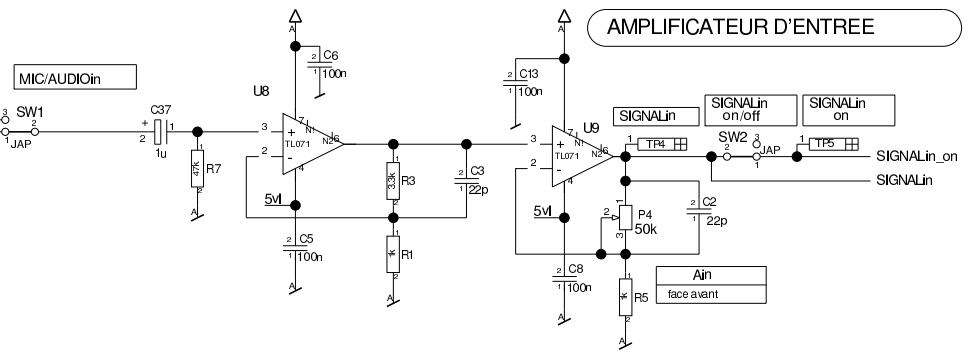
\includegraphics[width=.8\textwidth]{shema_echo_entree.png}
	\caption{Amplificateur d'entrée de la chambre d'écho}
	\label{fig:ampl}
\end{figure}

Dans la bande passante, on néglige les pertes dues au passe-bas C37-R7, car la fréquence de coupure vaut~:
${f_c = \frac{1}{2 \pi \cdot R_7 \cdot C_{37}} = 3,39 \mathrm{Hz}}$

De même, les capacités C2 et C3, et C5 et C8, peuvent être négligées et considérées comme des circuits ouverts.
En effet, au maximum de la bande passante ($f_{max} = 15 \mathrm{kHz}$) leur réactance vaut~:
\begin{center}$X_{c1,2} = \frac{1}{2 \pi f_{max} \cdot C_{2,3}} = 482 \mathrm{k\Omega} \gg R_3, P_4 $\end{center}
\begin{center}$X_{c5,8} = \frac{1}{2 \pi f_{max} \cdot C_{5,8}} = 106 \mathrm{\Omega} \gg R_1, R_5 $\end{center}

Le gain du premier étage est donc de : $A_1 \simeq 1+\frac{R3}{R1} = 4.3 $

Et le gain du second étage de :
$A_2 \simeq 1+\frac{\alpha P4}{R5}$, avec $\alpha \in [0,1]$~; soit~: $A_2 \in [1,51]$.

Le gain total $A = A_1\cdot A_2$ est donc compris entre $A_{min} = 4,3 = 12,7 \mathrm{dB}$ et $A_{max} = 219 = 46,8 \mathrm{dB}$.

\exsubpart{4}

Le rôle du séquenceur est de générer une fréquence d'horloge pour la logique numérique.

\begin{figure}[h]
	\centering
	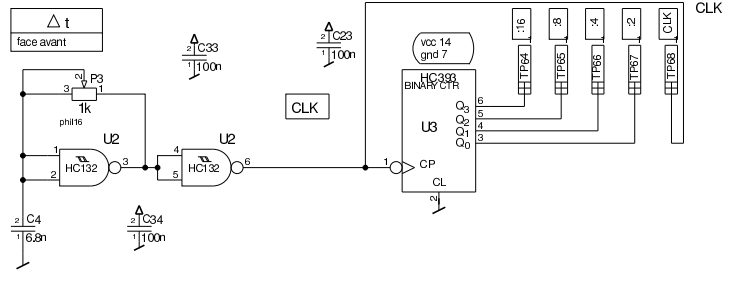
\includegraphics[width=.8\textwidth]{shema_sequenceur_1.png}
	\caption{Séquenceur de la chambre d'écho}
	\label{fig:seq}
\end{figure}

L'oscillateur est une simple cellule RC avec un inverseur à hystérésis.\\

D'après la notice du composant 74HC132, la fréquence d'oscillation quand elle est réglée au minimum (P3 réglé au maximum) est de :
\begin{center}
$f_{min} \simeq \frac{1}{0.8 \cdot R \cdot C} = 184 $ kHz
\end{center}

Le maximum est limité par le délai de propagation des transistors internes au circuit (lorsque $P3 = 0$), et est donc plus difficile à déterminer. Une grossière approximation est de prendre le temps de propagation du circuit, en ajoutant le temps de montée et de descente. Les valeurs typiques sont de 20 ns et 7 ns respectivement~:
\begin{center}
$f_{max} \simeq \frac{1}{tp_{lh} + tp_{hl} + t_{hl} + t_{lh}} = 18.5 $ MHz
\end{center}

P3 permet donc de faire varier librement la fréquence d'oscillation sur deux ordres de grandeur.

Le circuit U3 est un compteur, il permet donc d'avoir une version divisée de l'horloge par plusieurs puissances de 2. Dans ce cas, le compteur est sur 4 bits, il permet donc d'avoir un signal prédivisé par 2, 4, 8 et 16.
Nous pouvons choisir lequel de ces diviseurs est utilisé pour ce circuit ce qui permet de choisir grossièrement une très large bande de fréquences d'échantillonnage, en plus du réglage par P3.

Les deux bascules D de U19 forment un compteur Johnson de longueur 2, qui a 4 états. Le changement d'état se fait au flanc montant de CLK. \footnote{Voir datasheet du composant 74HC74}\\

\begin{figure}[h]
	\centering
	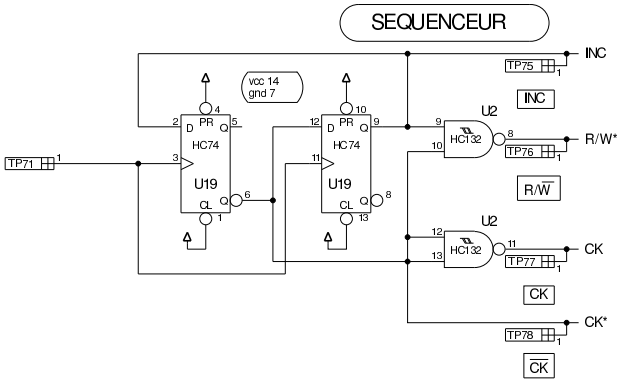
\includegraphics[width = 0.5\linewidth]{shema_sequenceur_2.png}
	\caption{Séquenceur de la chambre d'écho}
	\label{fig:seq2}
\end{figure}



Il y a donc un ``cycle'' pour chaque période de CK, soit 4 périodes de CLK. Chaque cycle se décompose donc en 4 phases bien distinctes\footnote{Voir schéma du montage et datasheets des composants respectifs : UVC3130 pour le convertisseur, 74HC4040 pour le contrôleur de bus d'adresses et 62256 pour la SRAM}~:
\begin{center}
\begin{tabular}{|c|c|c|c|c|c|l|}
\hline
\multicolumn{2}{|c|}{État} & CK & /CK & R/W & INC & Action\\
\hline
0 & 0 & 0 & 1 & 1 & 0 & Lecture de l'ancienne valeur par le convertisseur N/A (flanc descendant de CK) \\
%\hline
0 & 1 & 0 & 1 & 1 & 1 & Pas d'opération\\
%\hline
1 & 1 & 1 & 0 & 0 & 1 & Écriture de la nouvelle valeur dans la SRAM (état bas de R/W)\\
%\hline
1 & 0 & 1 & 0 & 1 & 0 & Mise-à-jour du bus d'adresses (flanc descendant de INC)\\
\hline
\end{tabular}
\end{center}

%Pas nécessaire...
%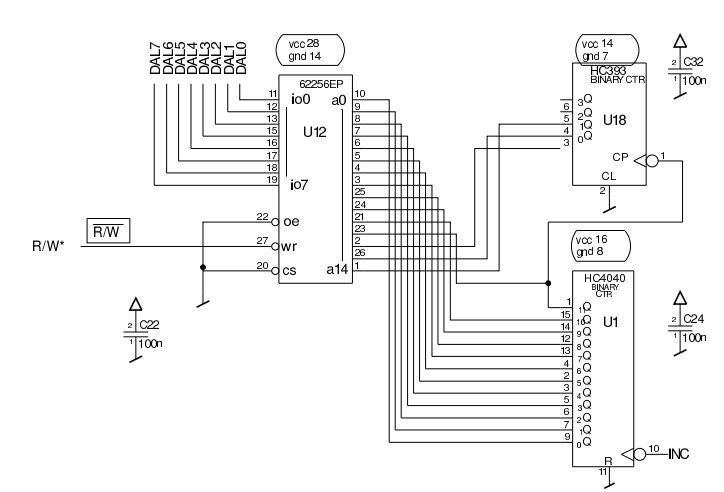
\includegraphics[width = 1\linewidth]{shema_memoire.png}

\begin{minipage}{0.5\linewidth}
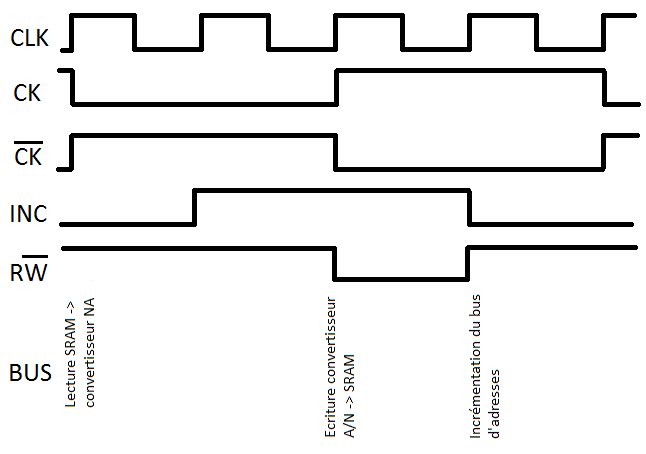
\includegraphics[width=\linewidth]{chronogramme_sequenceur.png}
\end{minipage}\hfill
\begin{minipage}{0.4\linewidth}
~~~~~~En conclusion~: À chaque cycle, une valeur dans la SRAM est d'abord lue et convertie en analogique, avant qu'une nouvelle valeur provenant du convertisseur A/N vienne remplacer cette valeur, puis on continue à l'adresse suivante.
\end{minipage}

\subsection{Mesures}

On applique en entrée de la chambre d'écho un signal sinusoïdal de 2kHz, et règle son amplitude ainsi que le gain du préamplificateur de la chambre d'écho de sorte à éviter toute saturation des convertisseurs A/N et N/A. 

Pour l'instant, on se place en mode ``écho seul''. Le signal en sortie n'est donc qu'une image quantifiée et retardée de l'entrée.

\exsubpart{2}

Afin d'observer plus clairement l'effet du filtre de lissage, on abaisse à 4 bits la résolution du CAN utilisé. Le résultat obtenu est présenté Fig.~\ref{fig:liss}.

\begin{figure}[h]
	\centering
	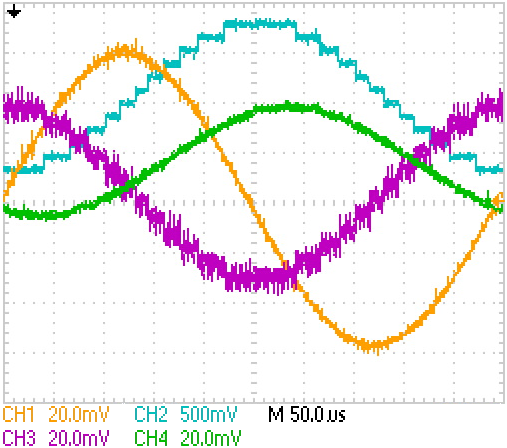
\includegraphics[width=.4\textwidth]{data/TEK0016_}
	\caption{\centering{Effet du filtre de lissage~:\\ CH1~: Entrée, CH2~: Sortie du CNA, \\CH4~: Sortie du filtre (après filtre de lissage)}}
	\label{fig:liss}
\end{figure}

On remarque qu'en l'absence de filtre (courbe bleu), les effets de la quantification sont très visible. En revanche, ils le sont moins après que le signal ait été traité par le filtre de lissage. En pratique, cela à pour effet de diminuer les harmoniques et le bruit créés par la quantification. Toutefois, il est impossible de les annuler tout à fait. En effet, le filtre de lissage doit être adapté à la plus forte pente envisageable pour une sortie idéale. Lorsque la pente est moindre, le lissage est alors imparfait.

\exsubpart{3}

À chaque bit supprimé pour l'encodage du signal traité, le niveau de bruit augmente de 6 dB. En effet, retirer un bit double l'amplitude de l'erreur de quantification.

% Il y a t-il des PHOTOS de l'analyseur de spectre pour mettre ici ?? %

\begin{figure}[h!]
	\centering
	\begin{subfigure}[b]{\textwidth}
		\begin{subfigure}[b]{.45\textwidth}
			\centering
			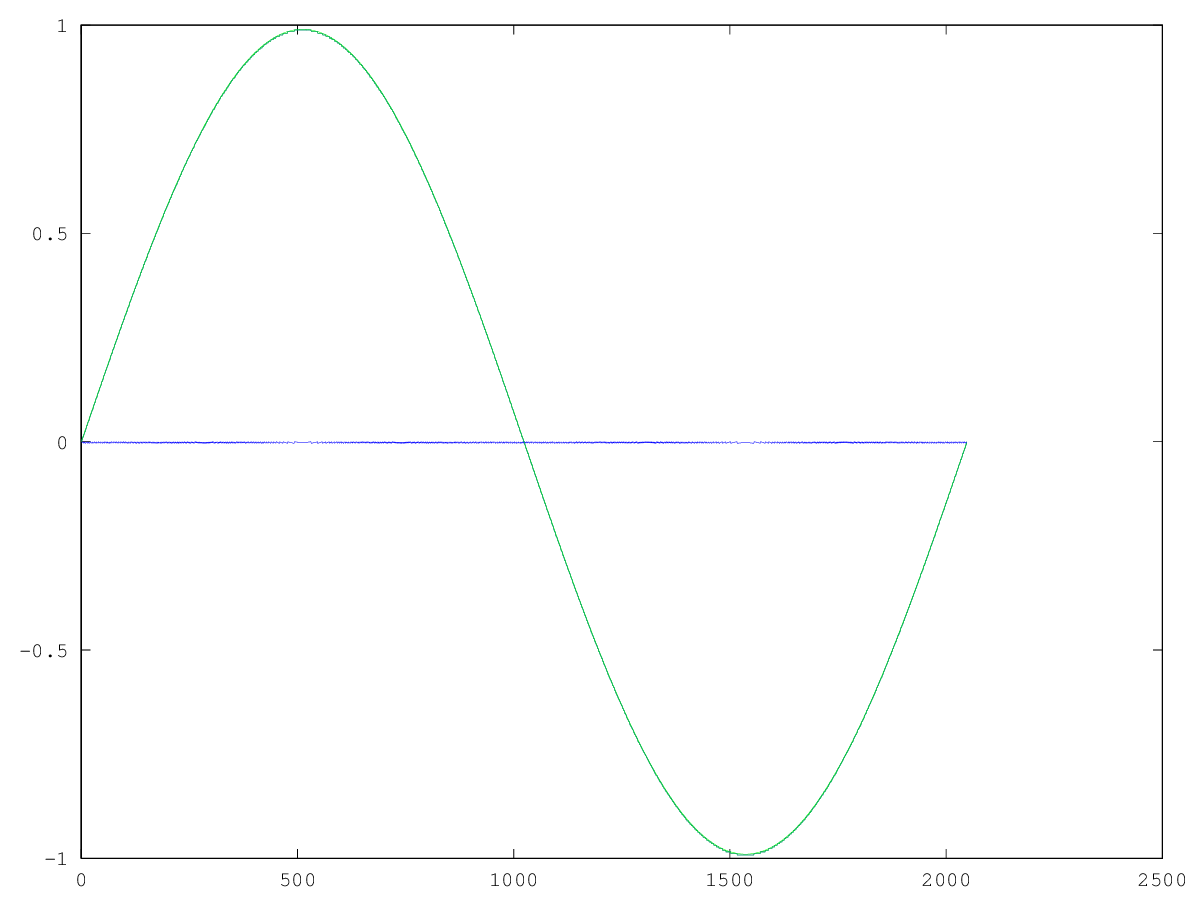
\includegraphics[width=\textwidth]{err_quantif_8bit_t}
			\caption{Sinus quantifié sur 8 bits et erreur}
			\label{fig:q_8a}
		\end{subfigure}
		\hfill
		\begin{subfigure}[b]{.45\textwidth}
			\centering
			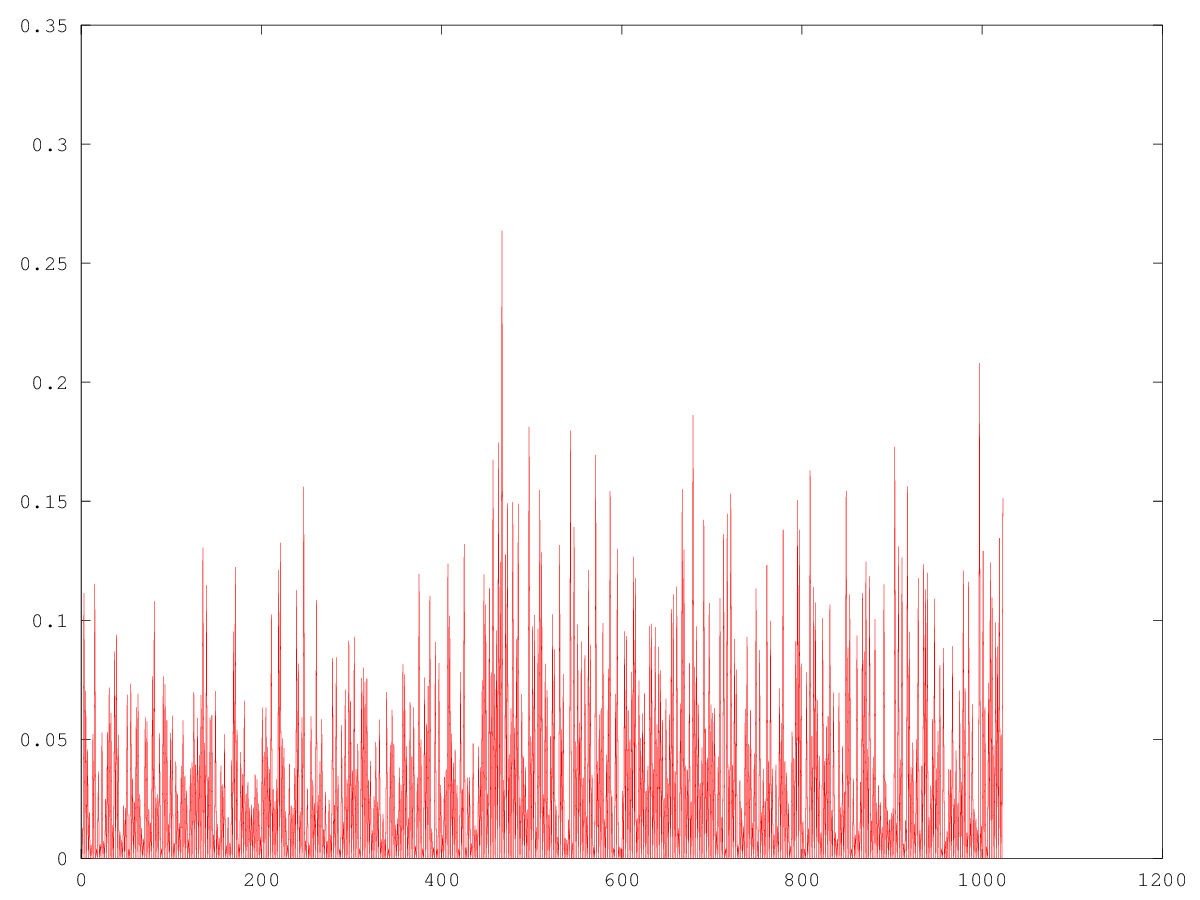
\includegraphics[width=\textwidth]{err_quantif_8bit_f}
			\caption{Spectre de l'erreur de quantification avec 8 bits}
			\label{fig:q_8b}
		\end{subfigure}
	\end{subfigure}
	\\
	\begin{subfigure}[b]{\textwidth}
		\begin{subfigure}[b]{.45\textwidth}
			\centering
			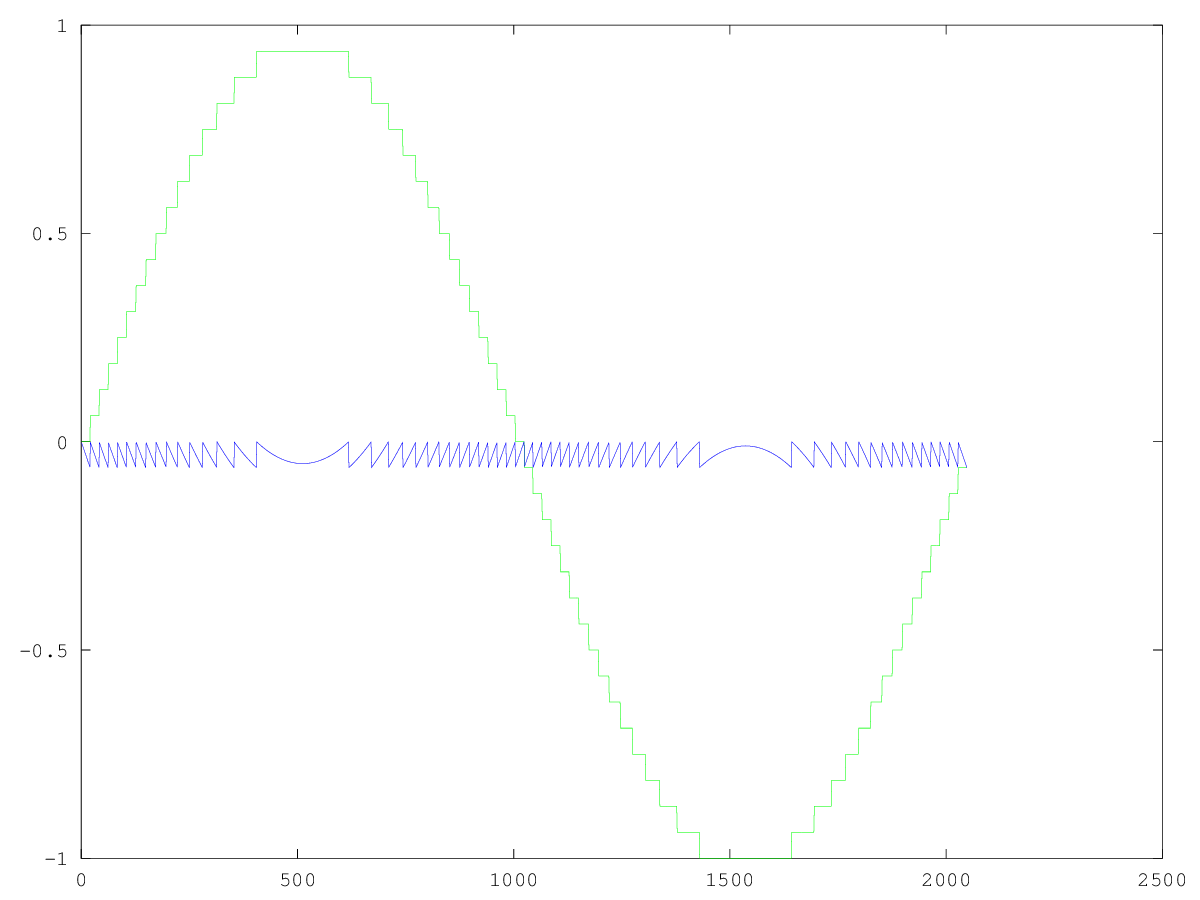
\includegraphics[width=\textwidth]{err_quantif_4bit_t}
			\caption{Sinus quantifié sur 4 bits et erreur}
			\label{fig:q_4a}
		\end{subfigure}
		\hfill
		\begin{subfigure}[b]{.45\textwidth}
			\centering
			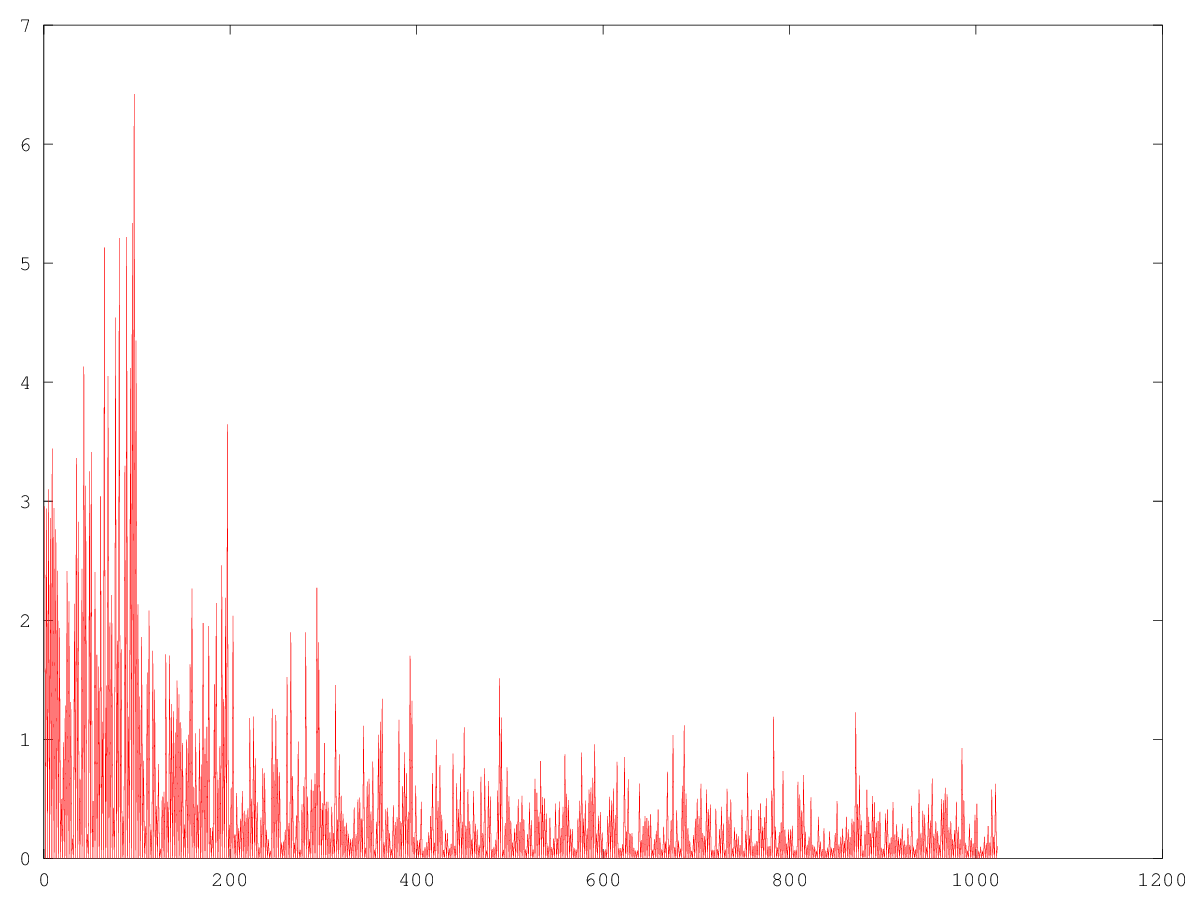
\includegraphics[width=\textwidth]{err_quantif_4bit_f}
			\caption{Spectre de l'erreur de quantification avec 4 bits}
			\label{fig:q_4b}
		\end{subfigure}
	\end{subfigure}
	\\
	\begin{subfigure}[b]{\textwidth}
		\begin{subfigure}[b]{.45\textwidth}
			\centering
			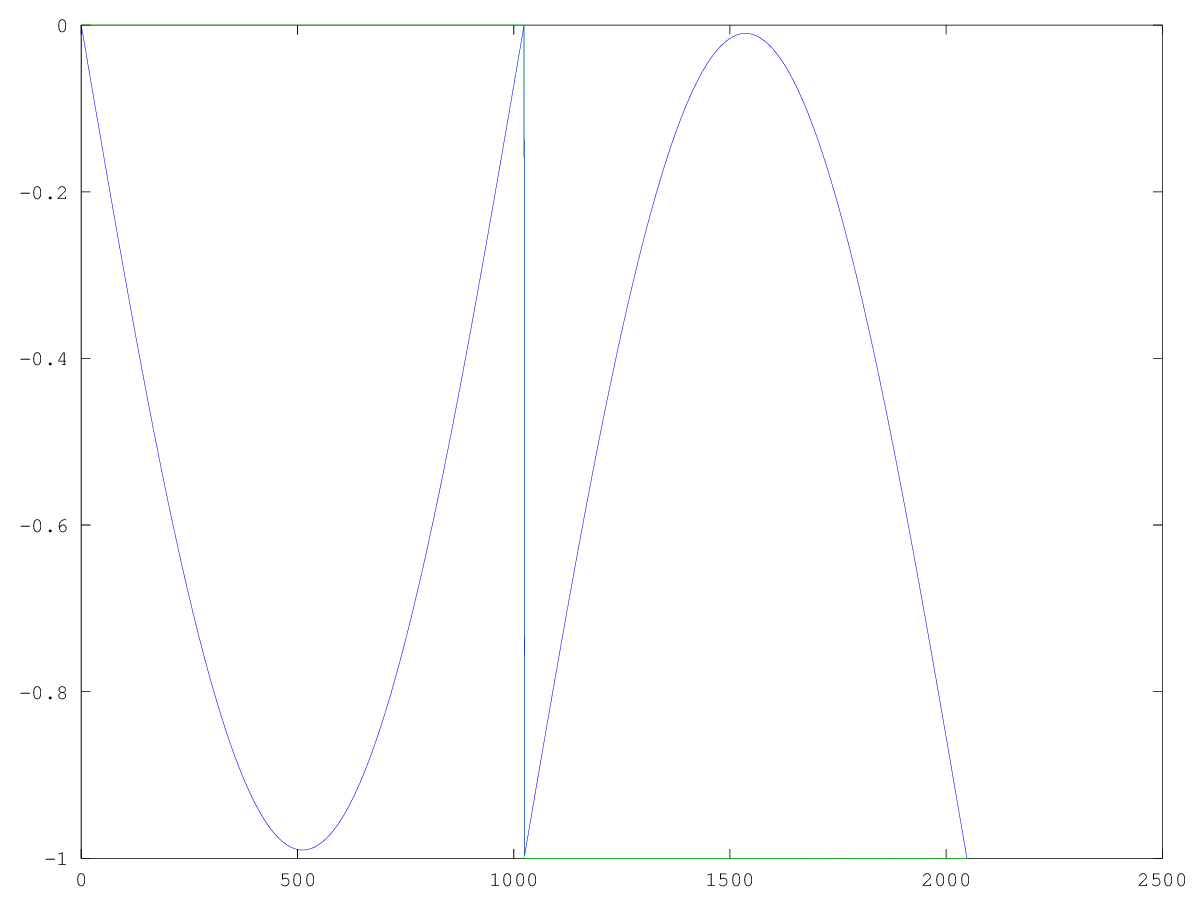
\includegraphics[width=\textwidth]{err_quantif_1bit_t}
			\caption{Sinus quantifié sur 1 bit et erreur}
			\label{fig:q_1a}
		\end{subfigure}
		\hfill
		\begin{subfigure}[b]{.45\textwidth}
			\centering
			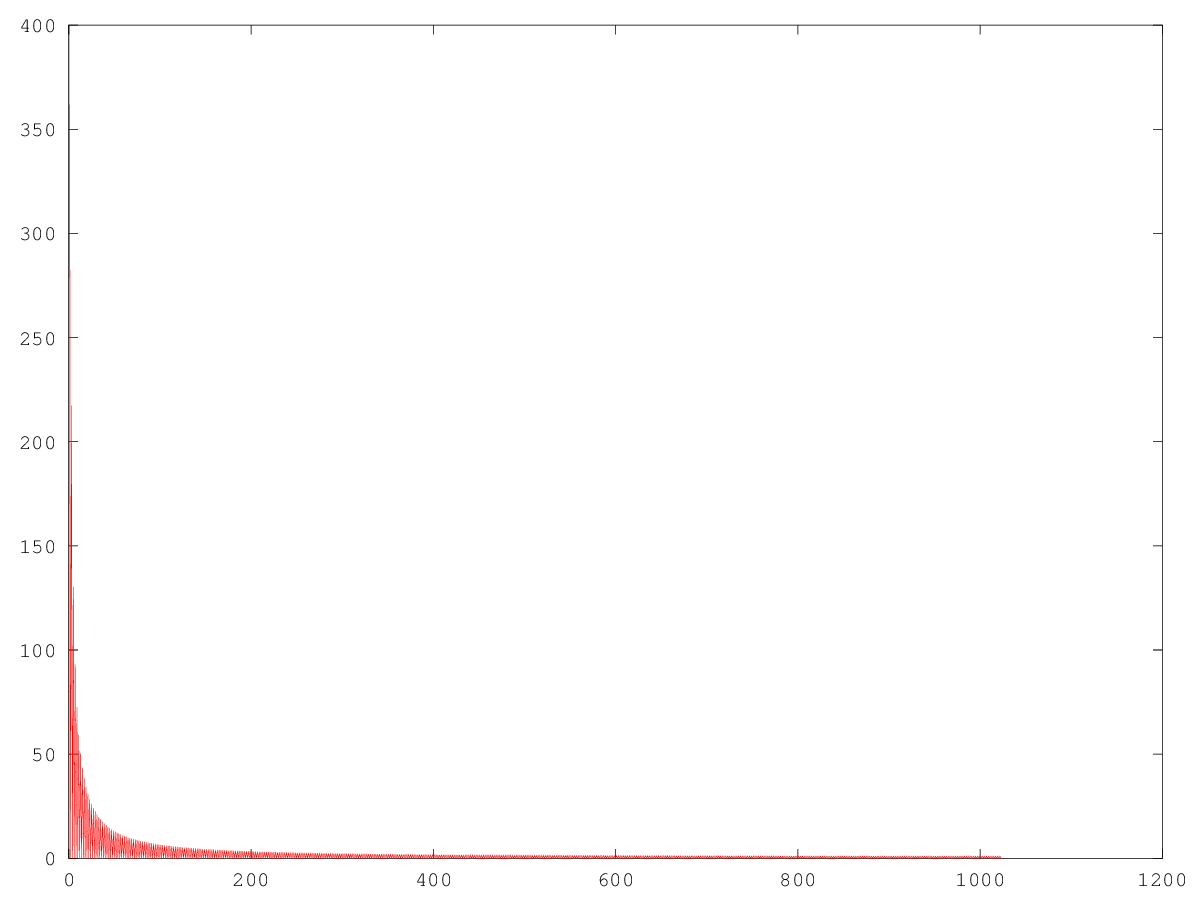
\includegraphics[width=\textwidth]{err_quantif_1bit_f}
			\caption{Spectre de l'erreur de quantification avec 1 bit}
			\label{fig:q_1b}
		\end{subfigure}
	\end{subfigure}	
	\caption{Effet du nombre de bits sur l'erreur de quantification\footnote{À noter que l'échelle sur l'axe des ordonnées n'est pas la même sur ces trois graphiques - à fin que ceux-ci soient observables.}}
\end{figure}


Concrètement, lorsque la résolution est suffisante --- c'est-à-dire le nombre de bits suffisant --- l'erreur de quantification peut être approximée comme étant aléatoire et apparait ainsi comme du bruit se superposant au signal traité. En revanche, lorsque le nombre de bits devient faible, la corrélation entre signal d'entré et bruit de quantification fait apparaitre des harmoniques. Le signal apparait alors comme fortement distordu.

Ainsi, avec 8 bits, l'erreur de quantification est répartie sur tout le spectre et peut être assimilée à du bruit blanc (cf Fig.~\ref{fig:q_8a} et~\ref{fig:q_8b}).
Avec 4 bits, on constate que l'erreur est plus intense en basse fréquence et présente certaines harmoniques (cf Fig.~\ref{fig:q_4a} et~\ref{fig:q_4b}).
Enfin, avec 1 bit, l'erreur correspond à la différence entre un signal sinusoïdal et un signal carré~: l'erreur est élevée et très condensée dans les basses fréquences --- et en aucun cas assimilable à du bruit blanc.

Nous avons branché un micro en entrée de la chambre d'écho. Dans le cas de la voix humaine, nous avons constaté qu'il faut au moins 4 bits pour qu'elle soit pleinement compréhensible.


\exsubpart{4}

On s'intéresse désormais au mode ``écho infini''.

Le retard à une influence sur la durée entre deux répétitions de l'écho. Un long retard pourra donner la sensation d'un écho plus lointain.
Le gain quant à lui a une influence sur l'atténuation entre deux répétitions de l'écho. Plus il sera élevé, plus l'on entendra l'écho avant que ce dernier ne se fonde dans le bruit.

Un retard long (supérieur à 0,2s) apparaitra comme un écho au sens classique du terme~: les sons apparaitront comme ``répétés''. En musique, on parle d'un effet de ``delay''. En revanche, si le retard est suffisamment court, il ne sera plus interprété comme tel, mais plutôt comme un effet de réverbération. On parle en musique de ``reverb''. Augmenter le gain rendra alors le son comme flou, pouvant ainsi le faire apparaitre comme plus calme, plus ésotérique\dots

Toutefois, le gain de l'écho ne doit jamais trop approcher 1, au risque de provoquer une saturation voire une instabilité du système.


\exsubpart{5}

Un taille de mémoire fixe permet de simplifier le contrôle des adresses mémoire~: un simple compteur modulo $2^n$ peut-être utilisé.

En revanche, il sera nécessaire d'avoir un circuit qui permet de faire varier la fréquence d'horloge pour l'échantillonnage. L'implémentation comme réalisée dans le séquenceur de ce montage convient parfaitement, mais ne permet pas un réglage précis de la fréquence d'échantillonnage. Si de la précision est requise, un oscillateur à quartz s'imposerait et il serait impossible de faire varier la fréquence de celui-ci. Il faudrait alors utiliser une PLL pour faire librement varier la fréquence ce qui est cher et compliqué à mettre en œuvre.

Autre effet indésirable~: si l'on change la longueur de l'écho durant le fonctionnement du circuit, la vitesse de lecture des données actuellement en mémoire sera affectée. Les fréquences des signaux correspondants seront ainsi transformées lors de leur lecture.
\\

Dans le cas d'une fréquence d'échantillonnage fixe, la génération de l'horloge est simplifiée, et pourrait être fabriquée de manière très précise à partir d'un quartz.

En revanche, le contrôle des adresses mémoire sera alors plus compliqué, nécessitant un décompteur qui recharge une variable lorsqu'il atteint la valeur zéro, la variable déterminant la longueur entre deux répétitions de l'écho.

Le changement de la longueur de l'écho pendant l'utilisation a un effet moindre sur la lecture des données en mémoire~: elles sont lues à la même vitesse, et aucun déplacement de fréquence n'est observé (pour peu que le retard soit assez grand devant la période des signaux). En revanche, on crée des trous ou raccourcit la séquence lue. Si le retard est élevé, on fera éventuellement entendre des bruits (``pops'') lorsque l'on arrive au bout du tampon mémoire. Si le retard est court, le son est distordu. 
Par ailleurs, il faut juste attendre que le compteur d'adresses atteigne la valeur `0' pour que le changement soit effectif.

\end{document}